\subsection{Detecting Signal Asynchrony Bugs}\label{sec:client-asynchrony}

\begin{figure}[tp]
    \hfill
    \begin{subfigure}[b]{.45\textwidth}
        \begin{subfigure}{\linewidth}
            \centering
            \begin{chisel}
val request           = Input(Bool())
val data              = Input(UInt(32.W))
val response          = Reg(UInt(32.W))
val valid             = Reg(Bool())
// --- Simplifed Design Logic ---
val buffered_response = Reg(UInt(32.W))
+ val buffered_valid  = Reg(Bool())
when (request) {
    buffered_response := data
}
response := buffered_response
- when (request) {
    -     valid := true.B
    - }
+ when (request) {
    +     buffered_valid := true.B
    + }
+ valid := buffered_valid
            \end{chisel}
            \caption{A bug-fixing commit for signal asynchrony.}
            \label{fig:asynchrony-code}
        \end{subfigure}

        \vspace{1ex}

        \begin{subfigure}{\linewidth}
            \centering
            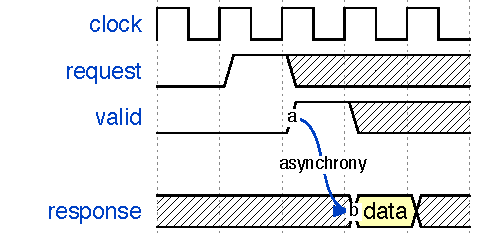
\includegraphics[width=\linewidth,clip,trim=20 0 10 0]{figures/asynchrony-waveform}
            \caption{Waveform illustrating the asynchrony between \texttt{valid} and \texttt{response} after a request.}
            \label{fig:asynchrony-waveform}
        \end{subfigure}
    \end{subfigure}
    \hfill
    \begin{subfigure}[b]{.53\textwidth}
        \begin{subfigure}{\linewidth}
            \centering
            \footnotesize
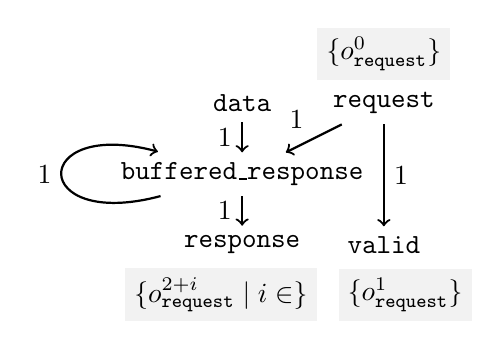
\begin{tikzpicture}[scale=.9,thick]
    \node (d) at (0, 0) {$\textpurple{\mathtt{data}}$};
    \node (rq) at (2, 0) {$\textpurple{\mathtt{request}}$};

    \node (br) at (0, -1) {$\mathtt{buffered\_response}$};
    \node (rp) at (0, -2) {$\mathtt{response}$};
    \node (v)  at (2, -2) {$\mathtt{valid}$};

    \draw[->] (d) -- node[left]{$1$} (br);
    \draw[->] (rq) -- node[above left]{$1$} (br);
    \draw[->] (br) edge[loop left] node{$1$} (br);
    \draw[->] (br) -- node[left]{$1$} (rp);
    \draw[->] (rq) -- node[right]{$1$} (v);


    \node[fill=gray!10] at (2, .7) {$\{o_{\mathtt{request}}^0\}$};
    \node[fill=gray!10] at (-.3, -2.7) {$\{o_{\mathtt{request}}^{2+i}\mid i\in\nats\}$};
    \node[fill=gray!10] at (2.3, -2.7) {$\{o_{\mathtt{request}}^1\}$};
\end{tikzpicture}

            \caption{\tia results before the bug fix, showing \emph{asynchronous} temporal influences of \texttt{request} on \texttt{response} and \texttt{valid}.}\label{fig:tia-asynchrony}
        \end{subfigure}

        \vspace{1ex}

        \begin{subfigure}{\linewidth}
            \centering
            \footnotesize
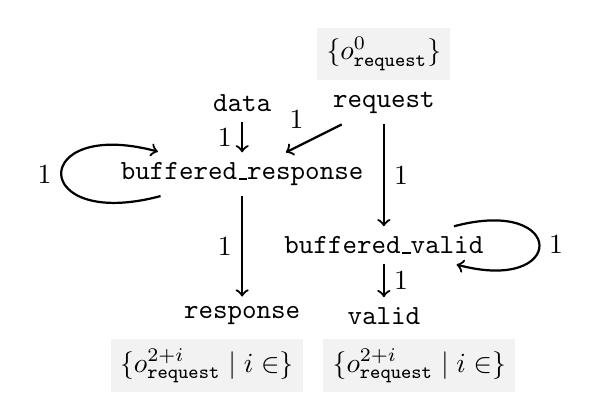
\begin{tikzpicture}[scale=.9,thick]
    \node (d) at (0, 0) {$\textpurple{\mathtt{data}}$};
    \node (rq) at (2, 0) {$\textpurple{\mathtt{request}}$};

    \node (br) at (0, -1) {$\mathtt{buffered\_response}$};
    \node (rp) at (0, -3) {$\mathtt{response}$};
    \node (bv)  at (2, -2) {$\mathtt{buffered\_valid}$};
    \node (v)  at (2, -3) {$\mathtt{valid}$};

    \draw[->] (d) -- node[left]{$1$} (br);
    \draw[->] (rq) -- node[above left]{$1$} (br);
    \draw[->] (br) edge[loop left] node{$1$} (br);
    \draw[->] (br) -- node[left]{$1$} (rp);
    \draw[->] (rq) -- node[right]{$1$} (bv);
    \draw[->] (bv) -- node[right]{$1$} (v);
    \draw[->] (bv) edge[loop right] node{$1$} (bv);


    \node[fill=gray!10] at (2, .7) {$\{o_{\mathtt{request}}^0\}$};
    \node[fill=gray!10] at (-.5, -3.7) {$\{o_{\mathtt{request}}^{2+i}\mid i\in\nats\}$};
    \node[fill=gray!10] at (2.5, -3.7) {$\{o_{\mathtt{request}}^{2+i}\mid i \in \nats\}$};
\end{tikzpicture}

            \caption{\tia results after the bug fix, showing \emph{synchronous} temporal influences of \texttt{request} on \texttt{response} and \texttt{valid}.}\label{fig:tia-synchrony}
        \end{subfigure}

        \vspace{1ex}

        \begin{subfigure}{\linewidth}
            \centering
            \footnotesize
            \[
            \begin{aligned}
                & \min\left\{i \mid o_{\mathtt{request}}^{i} \in \absT(\mathtt{response})\right\} \\
                \ne &\min\left\{i \mid o_{\mathtt{request}}^{i} \in \absT(\mathtt{valid})\right\} \\
            \end{aligned}
            \]
            \caption{An observation guiding signal asynchrony analysis.}
            \label{fig:asynchrony-observe}
        \end{subfigure}
    \end{subfigure}
    \hfill
    \caption{A motivating example for signal asynchrony analysis.}
\end{figure}

A \emph{signal asynchrony} bug occurs when two variables that are intended to be used together---such as a data variable and its associated valid or backpressure signal, or the two operands of a mathematical operation---are not updated synchronously~\cite{ma_debugging_2022}.
We'll first introduce signal asynchrony bugs through a simplified example and then describe how our signal asynchrony analysis detect such bugs leveraging the fundamental temporal influence information provided by \tia.

\paragraph{Example of A Signal Asynchrony Bug}

Figure~\ref{fig:asynchrony-code} shows a simplified Chisel example adapted from a bug-fixing commit~\cite{aysnchrony-fix-commit} for a signal asynchrony bug.
Deleted code is shown in red, while newly added code is shown in green.
The code describes a hardware design that responds to requests that requires a minimum two-cycle latency between each request (Line~1) and its corresponding response (Lines~3--4).
Upon receiving a request, the code therefore buffers the response, which can be computed in a single cycle, for one additional cycle in \texttt{buffered\_response} (Lines~8--10) before assigning it to the output \texttt{response} (Line~11).
However, in the buggy version, the \texttt{valid} signal, which indicates that \texttt{response} is valid, is asserted immediately upon receiving the request (Lines~12--14).
Consequently, \texttt{valid} becomes asserted one cycle before the corresponding \texttt{response} becomes valid, resulting in a signal asynchrony bug.
For simplicity, we omit the code that resets \texttt{valid} to 0.
Figure~\ref{fig:asynchrony-waveform} illustrates this asynchrony between \text{valid} and \text{response} after a request in the waveform.
The bug can be fixed by delaying \texttt{valid} by one cycle so that it becomes synchronized with \texttt{response}.
As shown in Figure~\ref{fig:asynchrony-code}, the developer introduces an intermediate register \texttt{buffered\_valid} (Line~7), assigns \texttt{valid} from it (Line~18), and replaces the original assignments to \texttt{valid} (Lines~12--14) with assignments to \texttt{buffered\_valid} (Lines~15--17).

\paragraph{Insights of Signal Asynchrony Analysis}

Figure~\ref{fig:tia-asynchrony} and Figure~\ref{fig:tia-synchrony} show the \tia results for the circuit in Figure~\ref{fig:asynchrony-code} before and after the signal asynchrony bug fix, respectively, focusing on how \texttt{request} temporally influences \texttt{response} and \texttt{valid}.
Before the fix, as shown in Figure~\ref{fig:tia-asynchrony}, the minimum temporal influence that \texttt{response} receives from \texttt{request} is two cycles, whereas that of \texttt{valid} is one cycle, indicating that the two signals are asynchronous with respect to \texttt{request}.
After the fix, as shown in Figure~\ref{fig:tia-synchrony}, both signals receive the same minimum temporal influence from \texttt{request}.
This observation is formally summarized in Figure~\ref{fig:asynchrony-observe}.

Guided by this observation, we generalize the \texttt{request} signal to an arbitrary synchronizer signal $p \in \ports$ and \texttt{response} and \texttt{valid} to arbitrary synchronized signals $x,y \in \variables$.
Our \emph{signal asynchrony analysis} reports that $x$ and $y$ are asynchronous with respect to $p$ if
\begin{equation}\label{eq:asynchrony}
    \min\left\{i \mid o_p^i \in \absT(x)\right\}
    \ne
    \min\left\{i \mid o_p^i \in \absT(y)\right\},
\end{equation}
where $\absT$ is the temporal influence information computed by \tia.

For practility, we compare the minimum temporal influences rather than the entire temporal influence sets in Equation~\ref{eq:asynchrony}.
In principle, comparing the entire sets would report asynchrony whenever the two signals have any difference in their temporal influence sets.
However, we observe in practice that this criterion is overly restrictive and kills many fine designs (i.e., falgs many false positive bugs), because two signals may have different temporal influence sets while still being sufficiently synchronized for their intended use.
The minimum temporal influence provides a simple and representative measure of when a signal can first become responsive to the synchronizer signal.
We therefore deliberately adopt this weaker criterion to reduce analysis noise and make the resulting reports more practical for hardware developers.

